

\documentclass[journal]{IEEEtran}

\usepackage{cite}
\usepackage{amsmath}
\interdisplaylinepenalty=2500
\usepackage{algorithm}
\usepackage[noend]{algpseudocode}
\usepackage{array}
\usepackage{graphicx}
\usepackage{float}

% correct bad hyphenation here
\hyphenation{op-tical net-works semi-conduc-tor}


\begin{document}
\title{Camera calibration using OpenCV}

\author{Wilbert~Pumacay,~\textit{Catholic University San Pablo},~wilbert.pumacay@ucsp.edu.pe\\
        Gerson~Vizcarra,~\textit{Catholic University San Pablo},~gerson.vizcarra@ucsp.edu.pe}

% make the title area
\maketitle

\begin{abstract}
Camera calibration is an important step in several applications, like augmented reality. To do calibration properly using current calibration methods we need to get features we can related in both 2D camera space and 3D world space to estimate the camera parameters that give this mapping. In this context, the use of grid patterns help by giving us the features we need, being the components in the pattern which we must detect in every frame in video.
\\
\\
In this paper we use Zhang \cite{CameraCalibration1} camera calibration technique implemented by OpenCV, and compare results using feature extraction of chessboard corners, symmetric/asymmetric circle grids, and concentric circle grid patterns, the first two, using funnctions implemented in OpenCV and the third one using our own algorithm by implementing a pipeline that gets these features by combining various techniques from classical image processing.
\end{abstract}

\begin{IEEEkeywords}
Camera calibration, calibration pattern, circle grid, image processing.
\end{IEEEkeywords}


\section{Introduction}

\IEEEPARstart{T}{he} camera calibration problem consists of finding 11 parameters that describe the mapping between 2D camera space and 3D world space. Six parameters, called extrinsic, come from an homogeneous transform, giving 6 parameters ( rotation and translation around the axes ). The other 5 parameters, called intrinsic, define some internal properties of the camera. This can be expressed in the following transformation equation:

\begin{equation}
  \begin{bmatrix}
    \mu \\
    \nu \\
      1 
  \end{bmatrix} = 
  \begin{bmatrix}
    \alpha & \gamma & \mu_{0} \\
       0   & \beta  & \nu_{0} \\
       0   &    0   &    1
  \end{bmatrix} 
  \begin{bmatrix}
    r_{x_{1}} & r_{y_{1}} & r_{z_{1}} & t_{x}\\
    r_{x_{2}} & r_{y_{2}} & r_{z_{2}} & t_{y}\\
    r_{x_{3}} & r_{y_{3}} & r_{z_{3}} & t_{z}
  \end{bmatrix} 
  \begin{bmatrix}
    x \\
    y \\
    z \\
    1
  \end{bmatrix}
%
\end{equation}

In this equation we can detail each of the variables: $x,y,z$ are original coordinates of an object, $r_{ij}$ and $t_{ij}$ means the rotation and translation values respectively in the model matrix, $\alpha$ and $\beta$ represents the focal length in x and y axis respectively, $\mu_0$ and $\nu_0$ are the coordinates x and y at the optical center.
\\
\\
To find these parameters, camera calibration methods make use of correspondences between 2D and 3D spaces in order to fit the parameters that best describe this mapping. We achieve this by minimizing the following function:

\begin{equation}
  \sum^{m}_{i} \sum^{n}_{j} \Vert TP^{ij}_{3D} - P^{ij}_{2D} \Vert^{2}
\end{equation}

Where we are trying to minimize the difference between the expected projection and the actual projection over some set of features. The key idea is that supplying sufficient features that have a correct mapping, we can get the 11 parameters needed that minimize this function. So, a key part is the detection of these features.
\\
\\
In equation $2$ we are looping through a set of features $n$ that are found in each frame of a video of $m$ frames, so, we basically need to detect some feature points in each frame of video, which is what we focus in this paper.

\section{About the method}
To compare results of feature extraction, we implemented the following pipeline.

\begin{figure}[H]
\centering
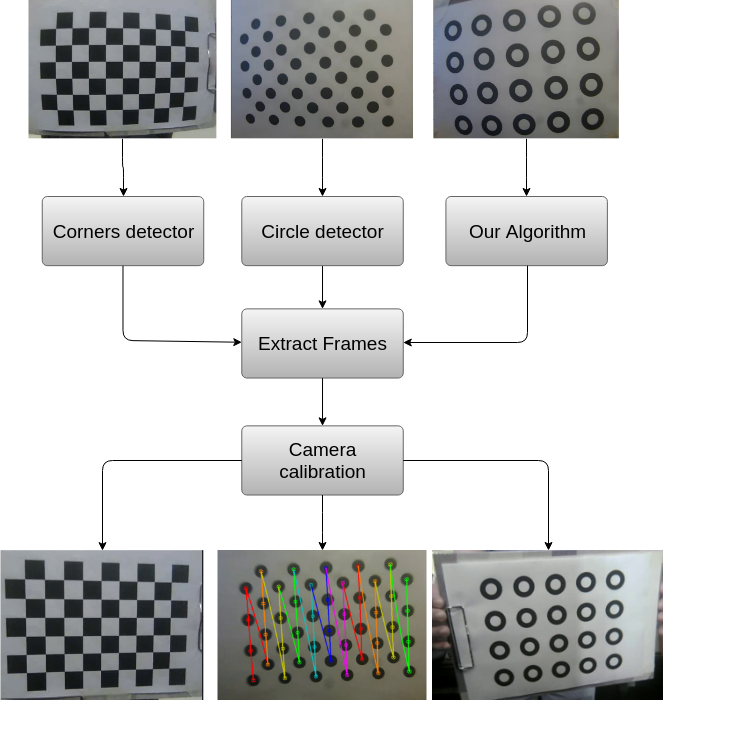
\includegraphics[width=2.5in]{_img/img_report3_pipeline.png}
\caption{Comparison pipeline.}
\end{figure}

\subsection{ Pattern detection }
We used three principal patterns to calibrate the camera with OpenCV calibration: Chessboard pattern, Circle symmetric/asymmetric pattern and circle concentric pattern. In the first two patterns we applied OpenCV implemented functions, in chessboard pattern we have to recognize corners and save their position, in circle pattern we have to detect circles and save the position of their centers.

\begin{figure}[H]
\centering
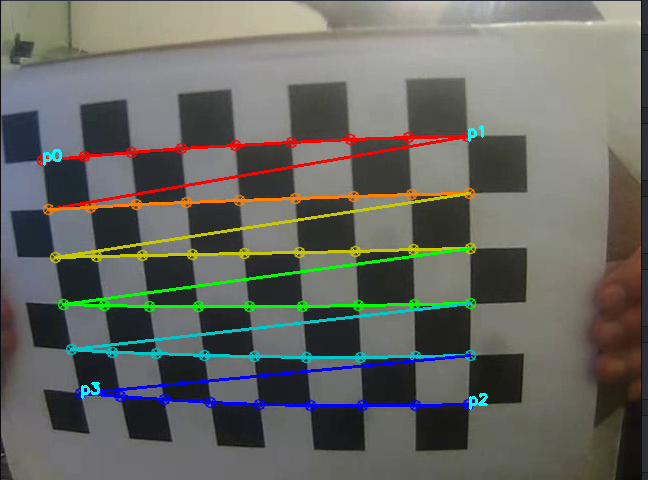
\includegraphics[width=2.5in]{_img/img_report3_detect_chessboard.png}
\caption{Chessboard pattern detection.}
\end{figure}
\begin{figure}[H]
\centering
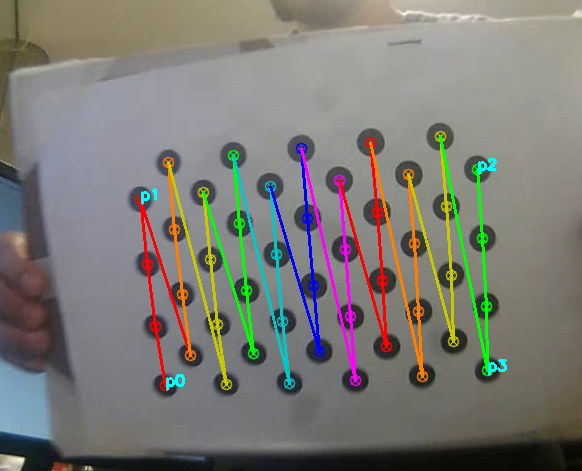
\includegraphics[width=2.5in]{_img/img_report3_detect_asymmetric.png}
\caption{Circle asymmetric grid pattern detection.}
\end{figure}


\subsection{ Circle concentric pattern detection}
The pipeline of our pattern detection and tracking algorithm works as follows:

\begin{figure}[H]
\centering
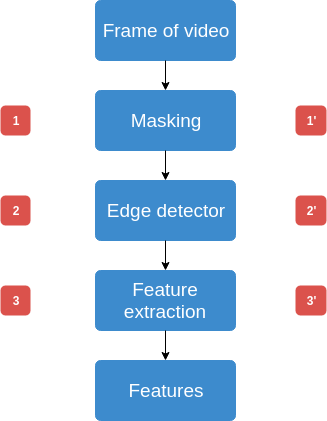
\includegraphics[width=2.5in]{_img/algorithm_overview.png}
\caption{Pipeline of previous work.}
\end{figure}

\subsubsection{ Use of ROI }
We setted a ROI (Region Of Interest) based on the firsts iterations, after we extract enough features on \textit{Feature extraction} stage, we used a ROI based on coordinates in features and a margin for predicting next frame features in order to reduce processing and avoid noise produced by ambient, we will apply next masking, edge detection, and feature extraction using ROI.
\\
\\
\begin{figure}[H]
\centering
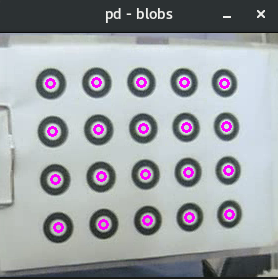
\includegraphics[width=2.5in]{_img/img_report2_processing_window.png}
\caption{ROI crop.}
\end{figure}

\subsubsection{ Masking }
This step is in charge of isolating the pattern by using threhsolding operations.
\\
\\
The approach consists on creating a mask from the grayscale transformed image applying \textbf{Adaptive Thresholding algorithm}, this algorithm relies on Integral Image technique especified in \cite{IntegralImageThresholding}.
\\
\\
%% TODO: Gerson
\begin{algorithm}
\caption{Masking}
\label{alg:mask2}
\begin{algorithmic}[1]
\State $\textit{Set up thresholding parameters}$
\State $mask   = \textit{rgb2gray}( inputImage )$
\State $mask   = \textit{AdaptiveThreshold}(mask, blockSize)$\\
\Return $masked$
\end{algorithmic}
\end{algorithm}
%%%%%%%%%%%%%%%%%%%%%%%%%%%%%%%%%%%%%%%%%%%%%%%%%%%%%%%

\begin{figure}[H]
\centering
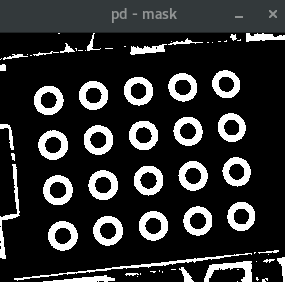
\includegraphics[width=2.5in]{_img/img_report2_mask.png}
\caption{Image mask applied to ROI.}
\end{figure}

\subsubsection{Edge detection}
In this stage of the pipeline we extract edges from the result of the previous stage. In order to do this, we applied \textbf{Scharr operators} on \textit{x} and \textit{y} axis (as described in algorithm 2); Scharr is the result from Sobel algorithm minimizing weighted mean squared angular error in Fourier domain.
%% TODO: Gerson
\begin{algorithm}
\caption{Edge detection}
\begin{algorithmic}[1]
\State $axis_x   = \textit{Scharr}(masked, 1, 0)$
\State $axis_x   = \textit{Abs}(axis_x)$
\State $axis_y   = \textit{Scharr}(masked, 0, 1)$
\State $axis_y   = \textit{Abs}(axis_y)$
\State $edgesImage   = \textit{Add}(axis_x, axis_y)$ \\
\Return $edgesImage$
\end{algorithmic}
\end{algorithm}

\begin{figure}[H]
\centering
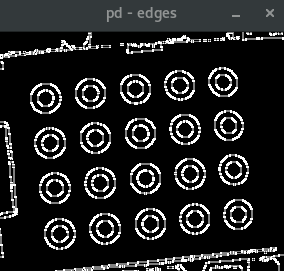
\includegraphics[width=2.5in]{_img/img_report2_edges.png}
\caption{Edge detection to mask.}
\end{figure}

\subsubsection{Feature extraction}
The last stage consist of extracting the features needed for the calibration from the edges detected in the previous stage. We used OpenCV's \textbf{SimpleBlobDetector} that apply an extra thresholding on image, applies the findContours algorithm calculating their centers, groups centers of several images by their coordinates in blobs, finally, estimates the final centers of blobs. For detecting only pattern blobs, we had to apply similar heuristics to avobe (color blobs, area, aspect ratio, and convexity of points) specified in \textit{Algorithm 3}.
\\
\\
%%%%%CHANGE THIS WILBERT%%%%%%
Also, in this stage we recognized the order of features detected. We started calculating the center of pattern given by the average coordinates of all features, then we computed features which are located in the corners of the pattern given by the farthest features from the center point. Next, we detected the vertical border points, selecting the nearest point to the line that pass through two corners. Similarly, we used border points to recognize the horizontal strips of points.
\\
\\ 
Finally, we used this information to give an ID number to every key point in pattern and store their location to track in next phase.
\\
\\
It should be noted that we only do recognition of features once, in next frames we only will extract features using \textit{SimpleBlobDetector} and track key points result in next step.
\\
\\
\begin{figure}[H]
\centering
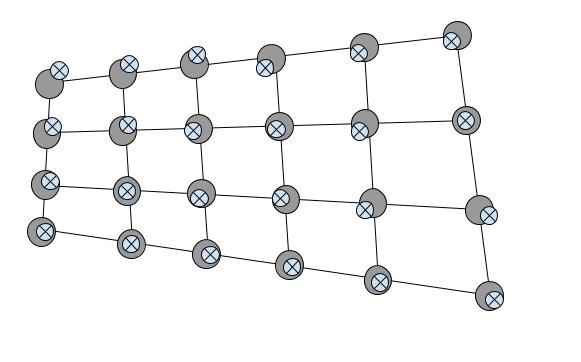
\includegraphics[width=2.5in]{_img/img_report3_pattern_matching.jpg}
\caption{Edge detection to mask.}
\end{figure}

\begin{figure}[H]
\centering
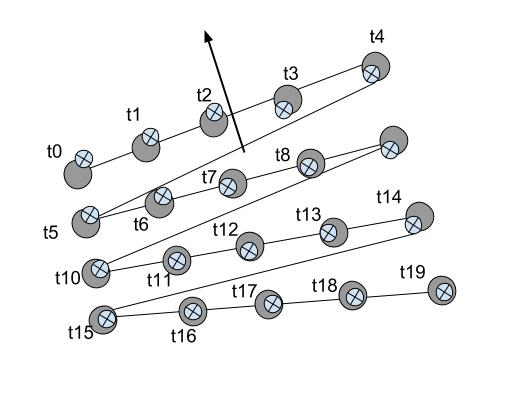
\includegraphics[width=2.5in]{_img/img_report3_pattern_order_check.jpg}
\caption{Edge detection to mask.}
\end{figure}

\begin{figure}[H]
\centering
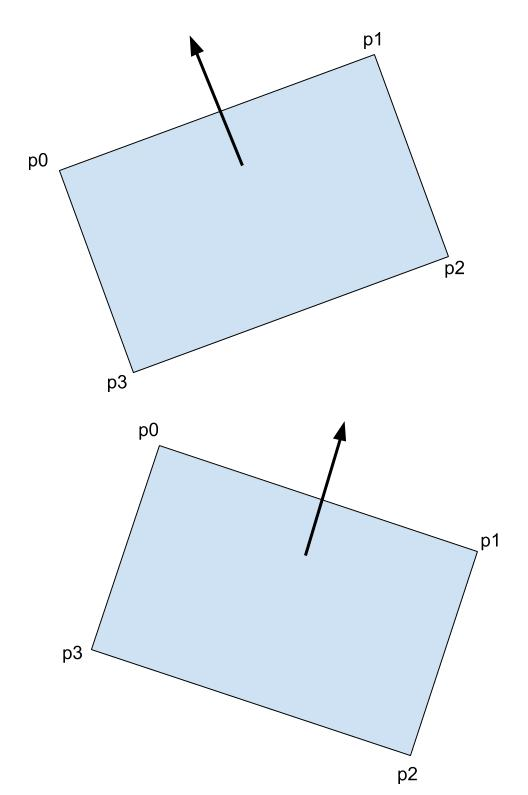
\includegraphics[width=2.5in]{_img/img_pattern_orientation_checking.jpg}
\caption{Edge detection to mask.}
\end{figure}

%% TODO: Gerson
\begin{algorithm}
\caption{Feature extraction}
\begin{algorithmic}[1]
\State $\textit{Set up detector parameters}$
\State $\textit{SimpleBlobDetector}(params)$
\State $keypoints   = \textit{detect}(mask)$ 
\State $midPt   = \textit{avg}(keypoints)$
\State $newKeypts[corners] = farthest(keypoints, midPt)$
\State $newKeypts[bord] = near(newKeypts[corners], keypoints)$
\State $newKeypts[rest] = near(newKeypts[bord], keypoints)$\\
\Return $newKeypts$
\end{algorithmic}
\end{algorithm}

\begin{figure}[H]
\centering
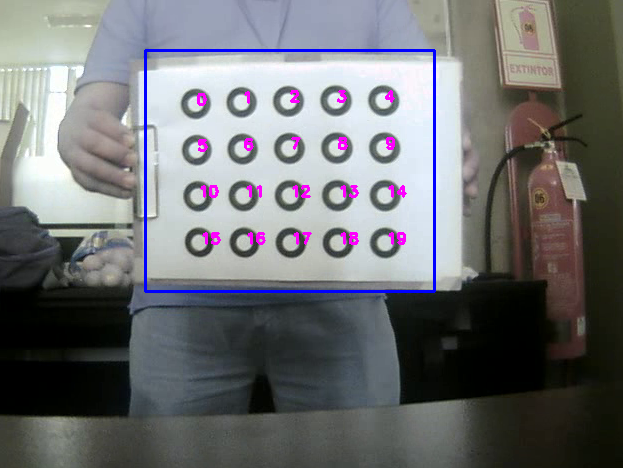
\includegraphics[width=2.5in]{_img/img_report2_feature_detection.png}
\caption{Result after feature detection.}
\end{figure}




\section{Results}
%todo wilbert

\section{Conclusions and Future improvements}
%todo wilbert

\IEEEtriggeratref{8}

% references section
\begin{thebibliography}{1}

\bibitem{OpenCV}
  Bradski, G. \\
  \textit{OpenCV library.} - 2000
\\
\bibitem{CameraCalibration1}
  Zhengyou Zhang \\
  \textit{A Flexible New Technique for Camera Calibration.} - 2000
\\
\bibitem{IntegralImageThresholding}
  Derek Bradley, Gerhard Roth \\
  \textit{Adaptive Thresholding Using the Integral Image.} - 2011

\end{thebibliography}


\end{document}

